\chapter{Garment Pick and Place Points}
\label{pick_and_place}
This chapter explains the last stage of our algorithm, in which the pick and place points required for unfolding the current fold are determined. These points will be later sent to the humanoid robot to perform the unfolding operation. This stage has as input the clustered depth map obtained in the clustering stage (described in chapter \ref{garment_clustering}), and the garment approximated polygon (calculated in section \ref{segmentation_approximated_polygon}). Figure \ref{fig:garment_pnp_points_blocks} shows the block diagram of the different steps that are performed in this stage.

\begin{figure}[thpb]
    \centering
    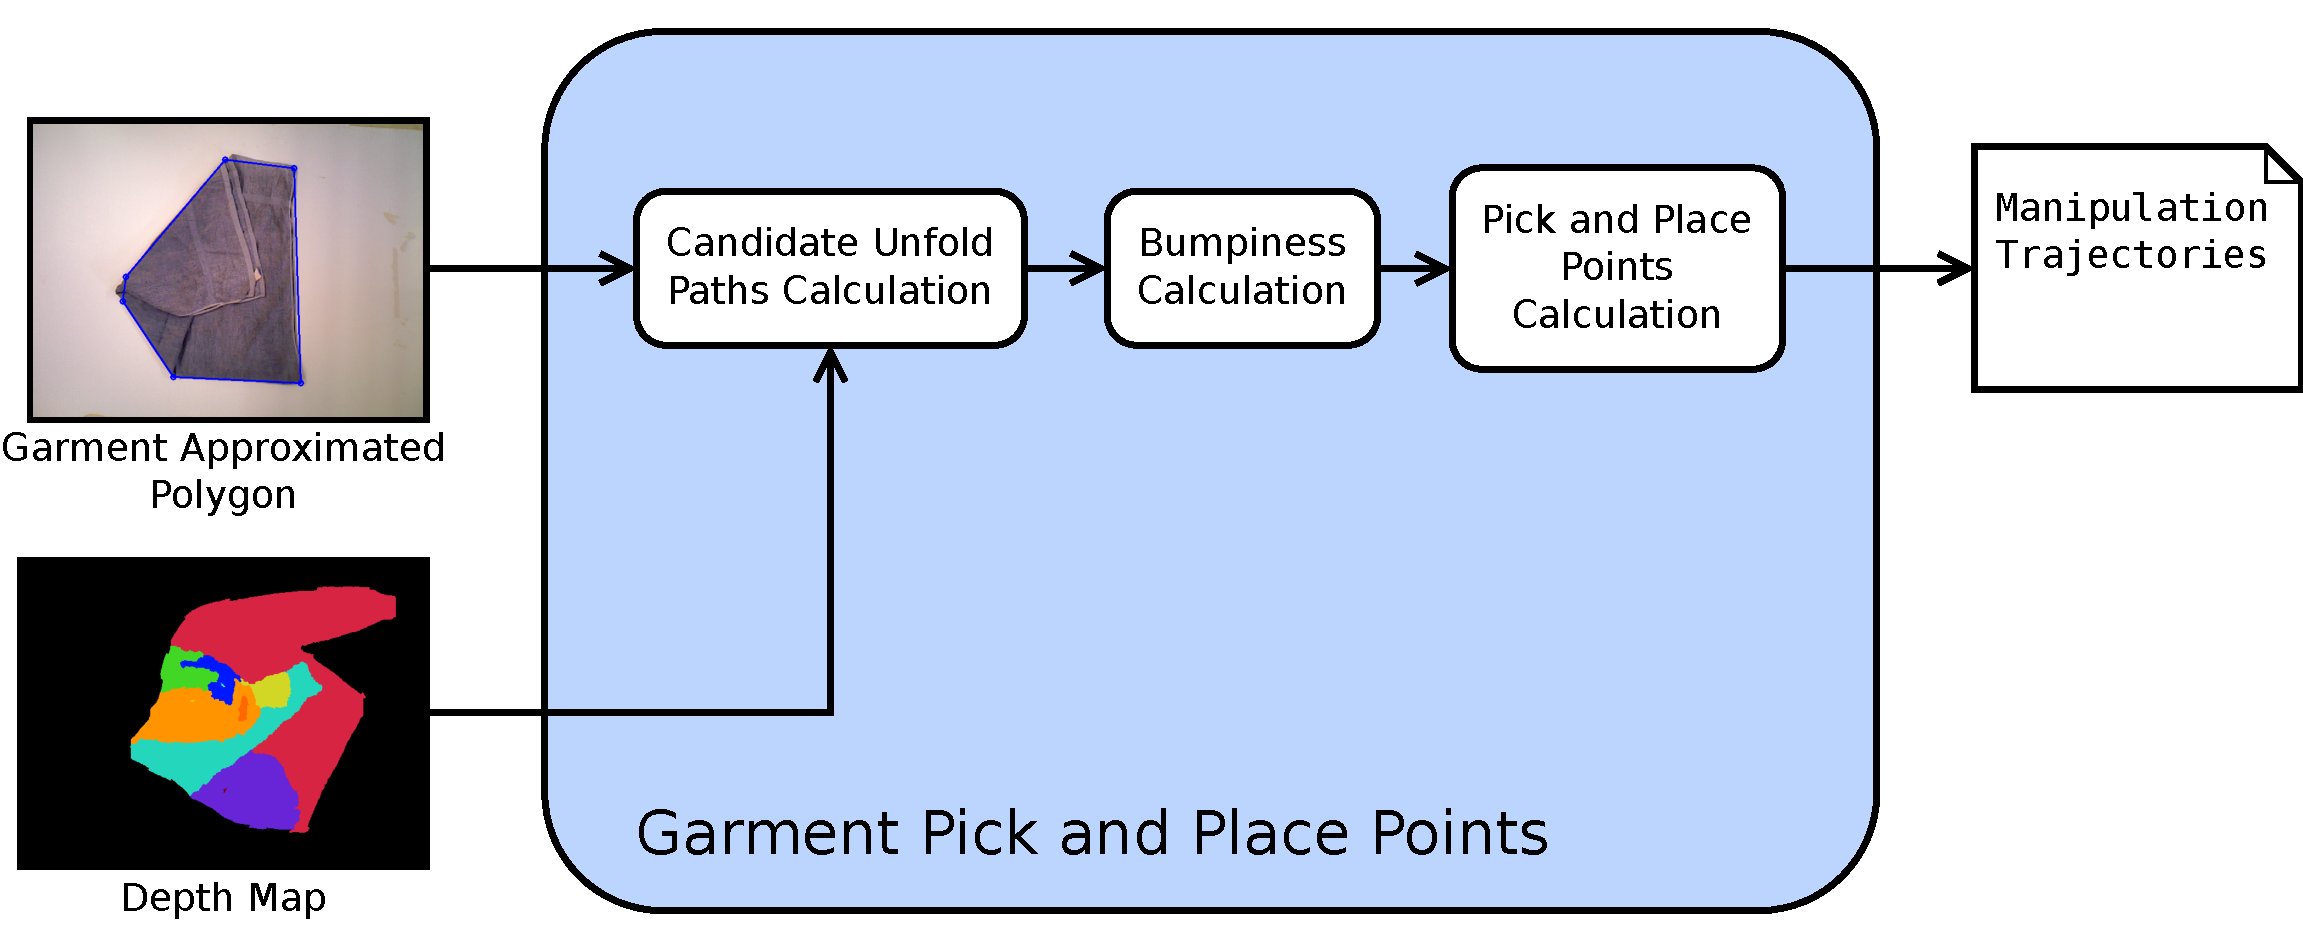
\includegraphics[width=\textwidth]
    {figures/Garment-pnp-points-diagram.pdf}
    \caption[Block diagram showing an overview of the Garment Pick and Place Points stage and its different steps.]
    {Block diagram showing an overview of the Garment Pick and Place Points stage and its different steps. The inputs for this stage are the garment approximated polygon, obtained in the Garment Segmentation stage, and the labeled cluster regions, obtained in the Garment Depth Map Clustering stage. After the analysis of these inputs, the most suitable manipulation trajectories are output to the robot to perform the unfolding action.}
    \label{fig:garment_pnp_points_blocks}
\end{figure}

\section{Candidate Unfold Paths}
\label{pnp:unfold_paths}

Based on the assumption that when a garment has an overlapping fold, the fold line will rest on the garment contour, and the folded surface will have lower depth values (i.e. closer to the depth sensor), the next step in our algorithm is to create a set of paths from the highest point of the garment to the midpoint of each contour segment. These paths will be later analyzed using the clusters previously found in the depth image to select the path with less height variation.

To find the highest point in the garment, the clusters previously found with the Watershed algorithm are averaged using the median value for each cluster. Then, the region with the lowest depth value, which is closest to the camera and therefore highest in the garment, is selected as overlapping fold based on the previous assumption. The centroid of the selected cluster is the point selected as the highest point. Using this method instead of selecting directly the highest point from the depth image increases the robustness of the algorithm against outliers and noise present in the depth image.

The midpoint of each segment of the garment approximated polygon is then calculated, and a set of paths departing from the highest point and arriving to the midpoints is created.

These paths are checked so that they are located entirely inside the garment. Paths that go outside the garment approximated polygon are considered invalid. Figure \ref{fig:candidate_paths} shows both the initial paths set and the unfold candidate paths set, without the invalid paths.


\begin{figure}[htbp]
	\centering
    \begin{subfigure}[l]{0.49\textwidth}
	    \centering
    	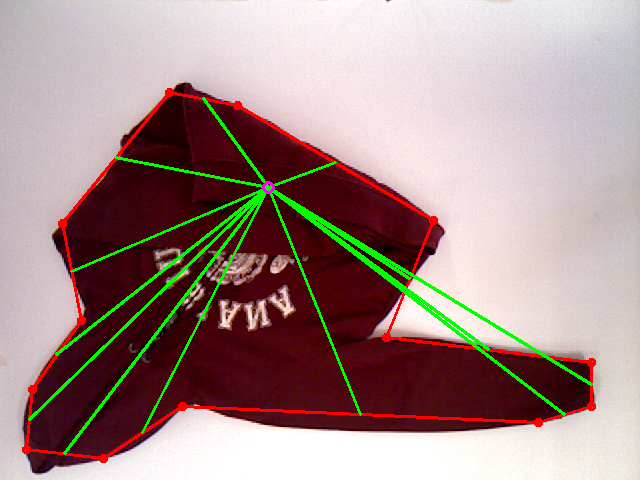
\includegraphics[width=\textwidth]
    	{figures/paths_candidate.png}
    	\caption{Set of candidate paths}
	\end{subfigure}
	~
    \begin{subfigure}[r]{0.49\textwidth}
	    \centering
    	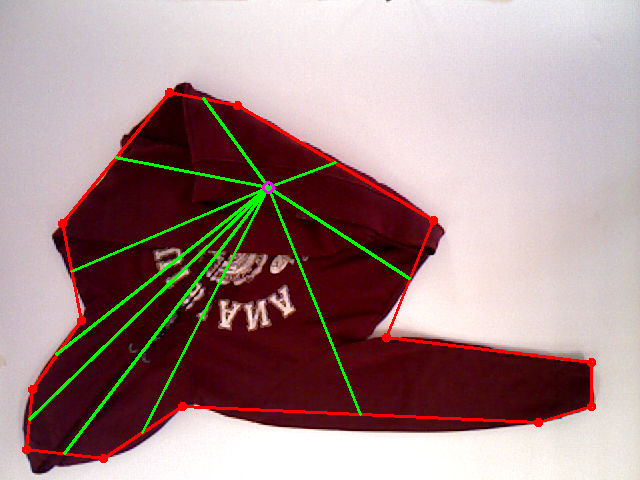
\includegraphics[width=\textwidth]
    	{figures/paths_valid.png}
    	\caption{Set of valid paths}
	\end{subfigure} 
    \caption[Initial candidate paths and valid set of paths.]
    {The left image displays the set of initial candidate paths (green lines) to be used as unfolding directions. These paths are generated starting at the centroid of the highest region, represented with a magenta circle, and ending at the midpoint of each of the edges of the approximated garment polygon, shown in red lines. These paths are filtered, and the resulting valid paths, that do not cross the outer approximated polygon, are shown in the right figure.}
    \label{fig:candidate_paths}
\end{figure}


\section{Bumpiness}
\label{pnp:bumpiness}
Each of the candidate paths calculated using the method explained in the previous section has to be analyzed in this step to determine the best unfolding path. 

We can represent each of the $n$ candidate paths obtained as a 2D parametric line ($\mathbb{R} \to \mathbb{R}^2$) depending on a parameter $r$, the radial distance to the highest point:

\begin{equation}
\textrm{path}(r) = \left[u(r), v(r)\right]
\end{equation}

Where $u$ and $v$ are pixel coordinates in the image frame of reference.

Prior to the analysis, each of the paths of length $L$ is discretized in segments with a constant length $l$. The depth image $\mathcal{D}(u,v)$ is sampled at those discrete points. This results in $n$ ordered sets $S=\{ s_1,...,s_m\}$ of depth samples to be analyzed, where:


\begin{equation}
s_i = \mathcal{D}(path(i \cdot l)), \quad  i=0,1,2,..., m
\end{equation}

As the different paths may differ in length $L$, the amount of sampled points ($m=${\Large$\lfloor\frac{L}{l}\rfloor$}) will be different for each path. Figure \ref{fig:paths_with_bumpiness} shows the sample set $S$ corresponding to each candidate path for a certain garment example.

The differences in depth between the overlapping fold region and the rest of the clothing article are assumed to be greater than the diferences in depth within the fold region points. Under that assumption, the metric to evaluate the best path is a \textit{bumpiness} value \textit{B}, which is calculated by penalizing the changes in depth along each of the $n$ candidate sample sets $S$, as shown in Equation \ref{eq:bumpiness}.

\begin{equation}\label{eq:bumpiness}
B = \sum_{i=2}^{m} | s_i- s_{i-1} | 
\end{equation}

The candidate set with the lowest bumpiness value, which corresponds to the path with the least and smallest height changes, is selected as the unfold direction, as shown in Figure \ref{fig:paths_with_bumpiness}.

\begin{figure}[thpb]
    \centering
    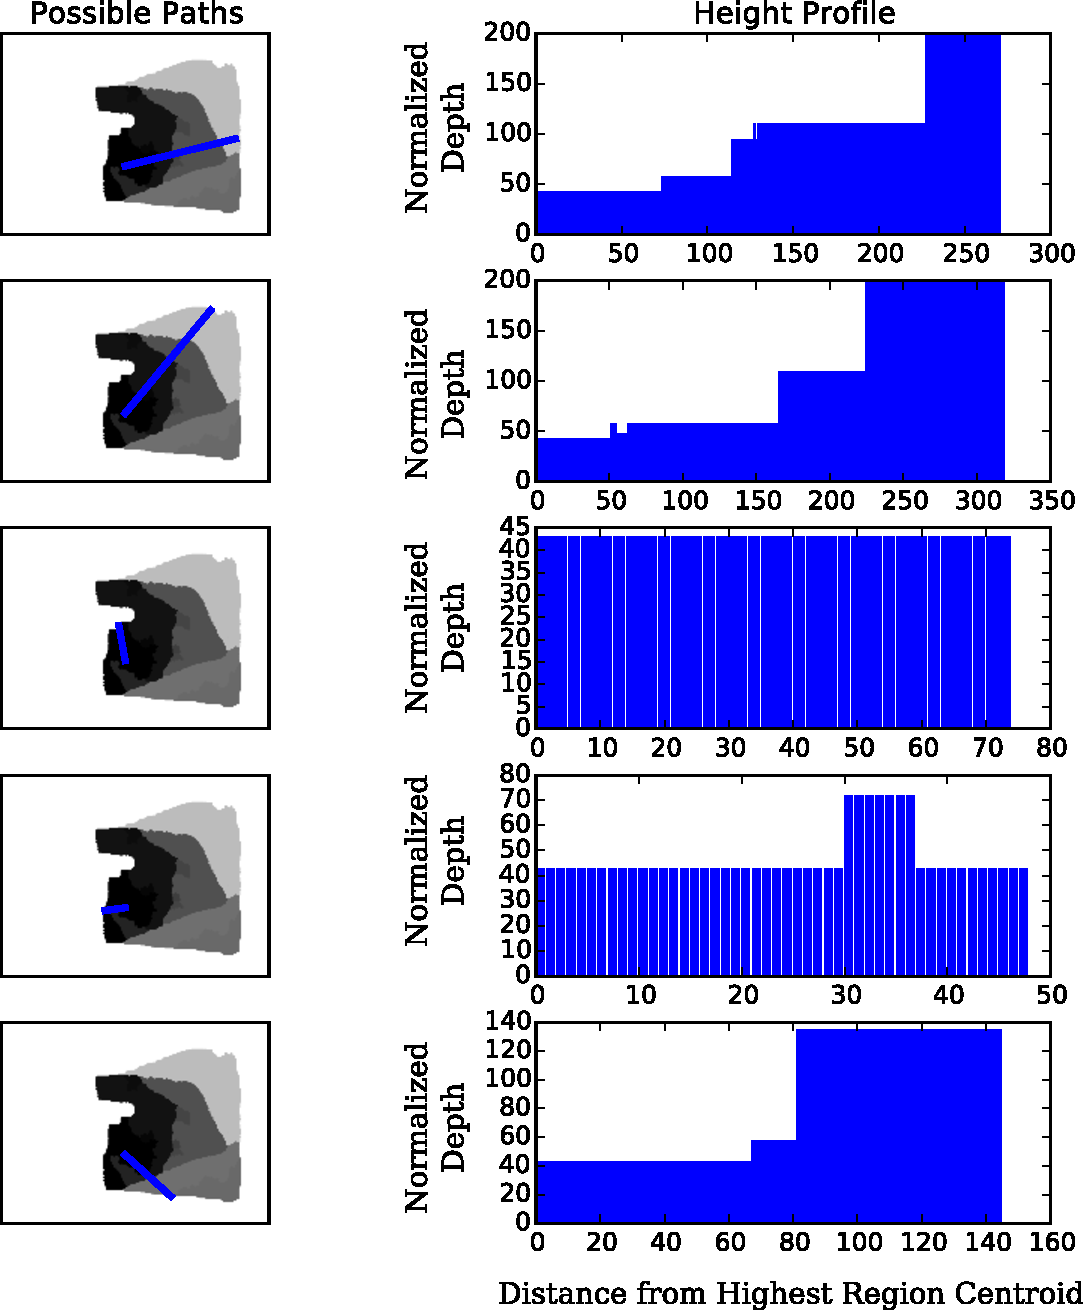
\includegraphics[width=\textwidth]{figures/candidate_paths.pdf}
    \caption[Bumpiness along several candidate paths.]
    {On the left side, the candidate paths are shown. On the right side, the height profile of each path is shown. Note that the depth sensor computes the distance to the object from itself, so that a low value in the bar plot means a closer object to the sensor, and therefore it is a region with more height with respect to the table. The highlighted path is the one with the lowest value of bumpiness, and it is selected as suitable unfolding path.}
    \label{fig:paths_with_bumpiness}
\end{figure}

\section{Pick and Place Points}
\label{pnp:pick_and_place}
Once the most promising path for unfolding has been identified, the last step is to obtain pick and place points for the robot to perform the unfold action. Due to the absence of a cuantitative metric for determining the suitability of those points, the point selection criteria has been selected using intuition from all possible choices.

The selected grasping point for the picking action is located at the intersection between the unfolding path direction line and the highest garment region border. This point is obtained by calculating the intersection between the selected path line and the highest region contour. This operation results in two intersection points, from which the furthest to the garment border is selected.

The other point is used as axis for a point reflection. To find the placing point, a reflection transformation is applied to the picking point using the aforementioned point as axis. Figure \ref{fig:directions} shows the unfold directions for several clothes, departing at the picking points and arriving to the placing points.

\begin{figure}[thpb]
    \centering
    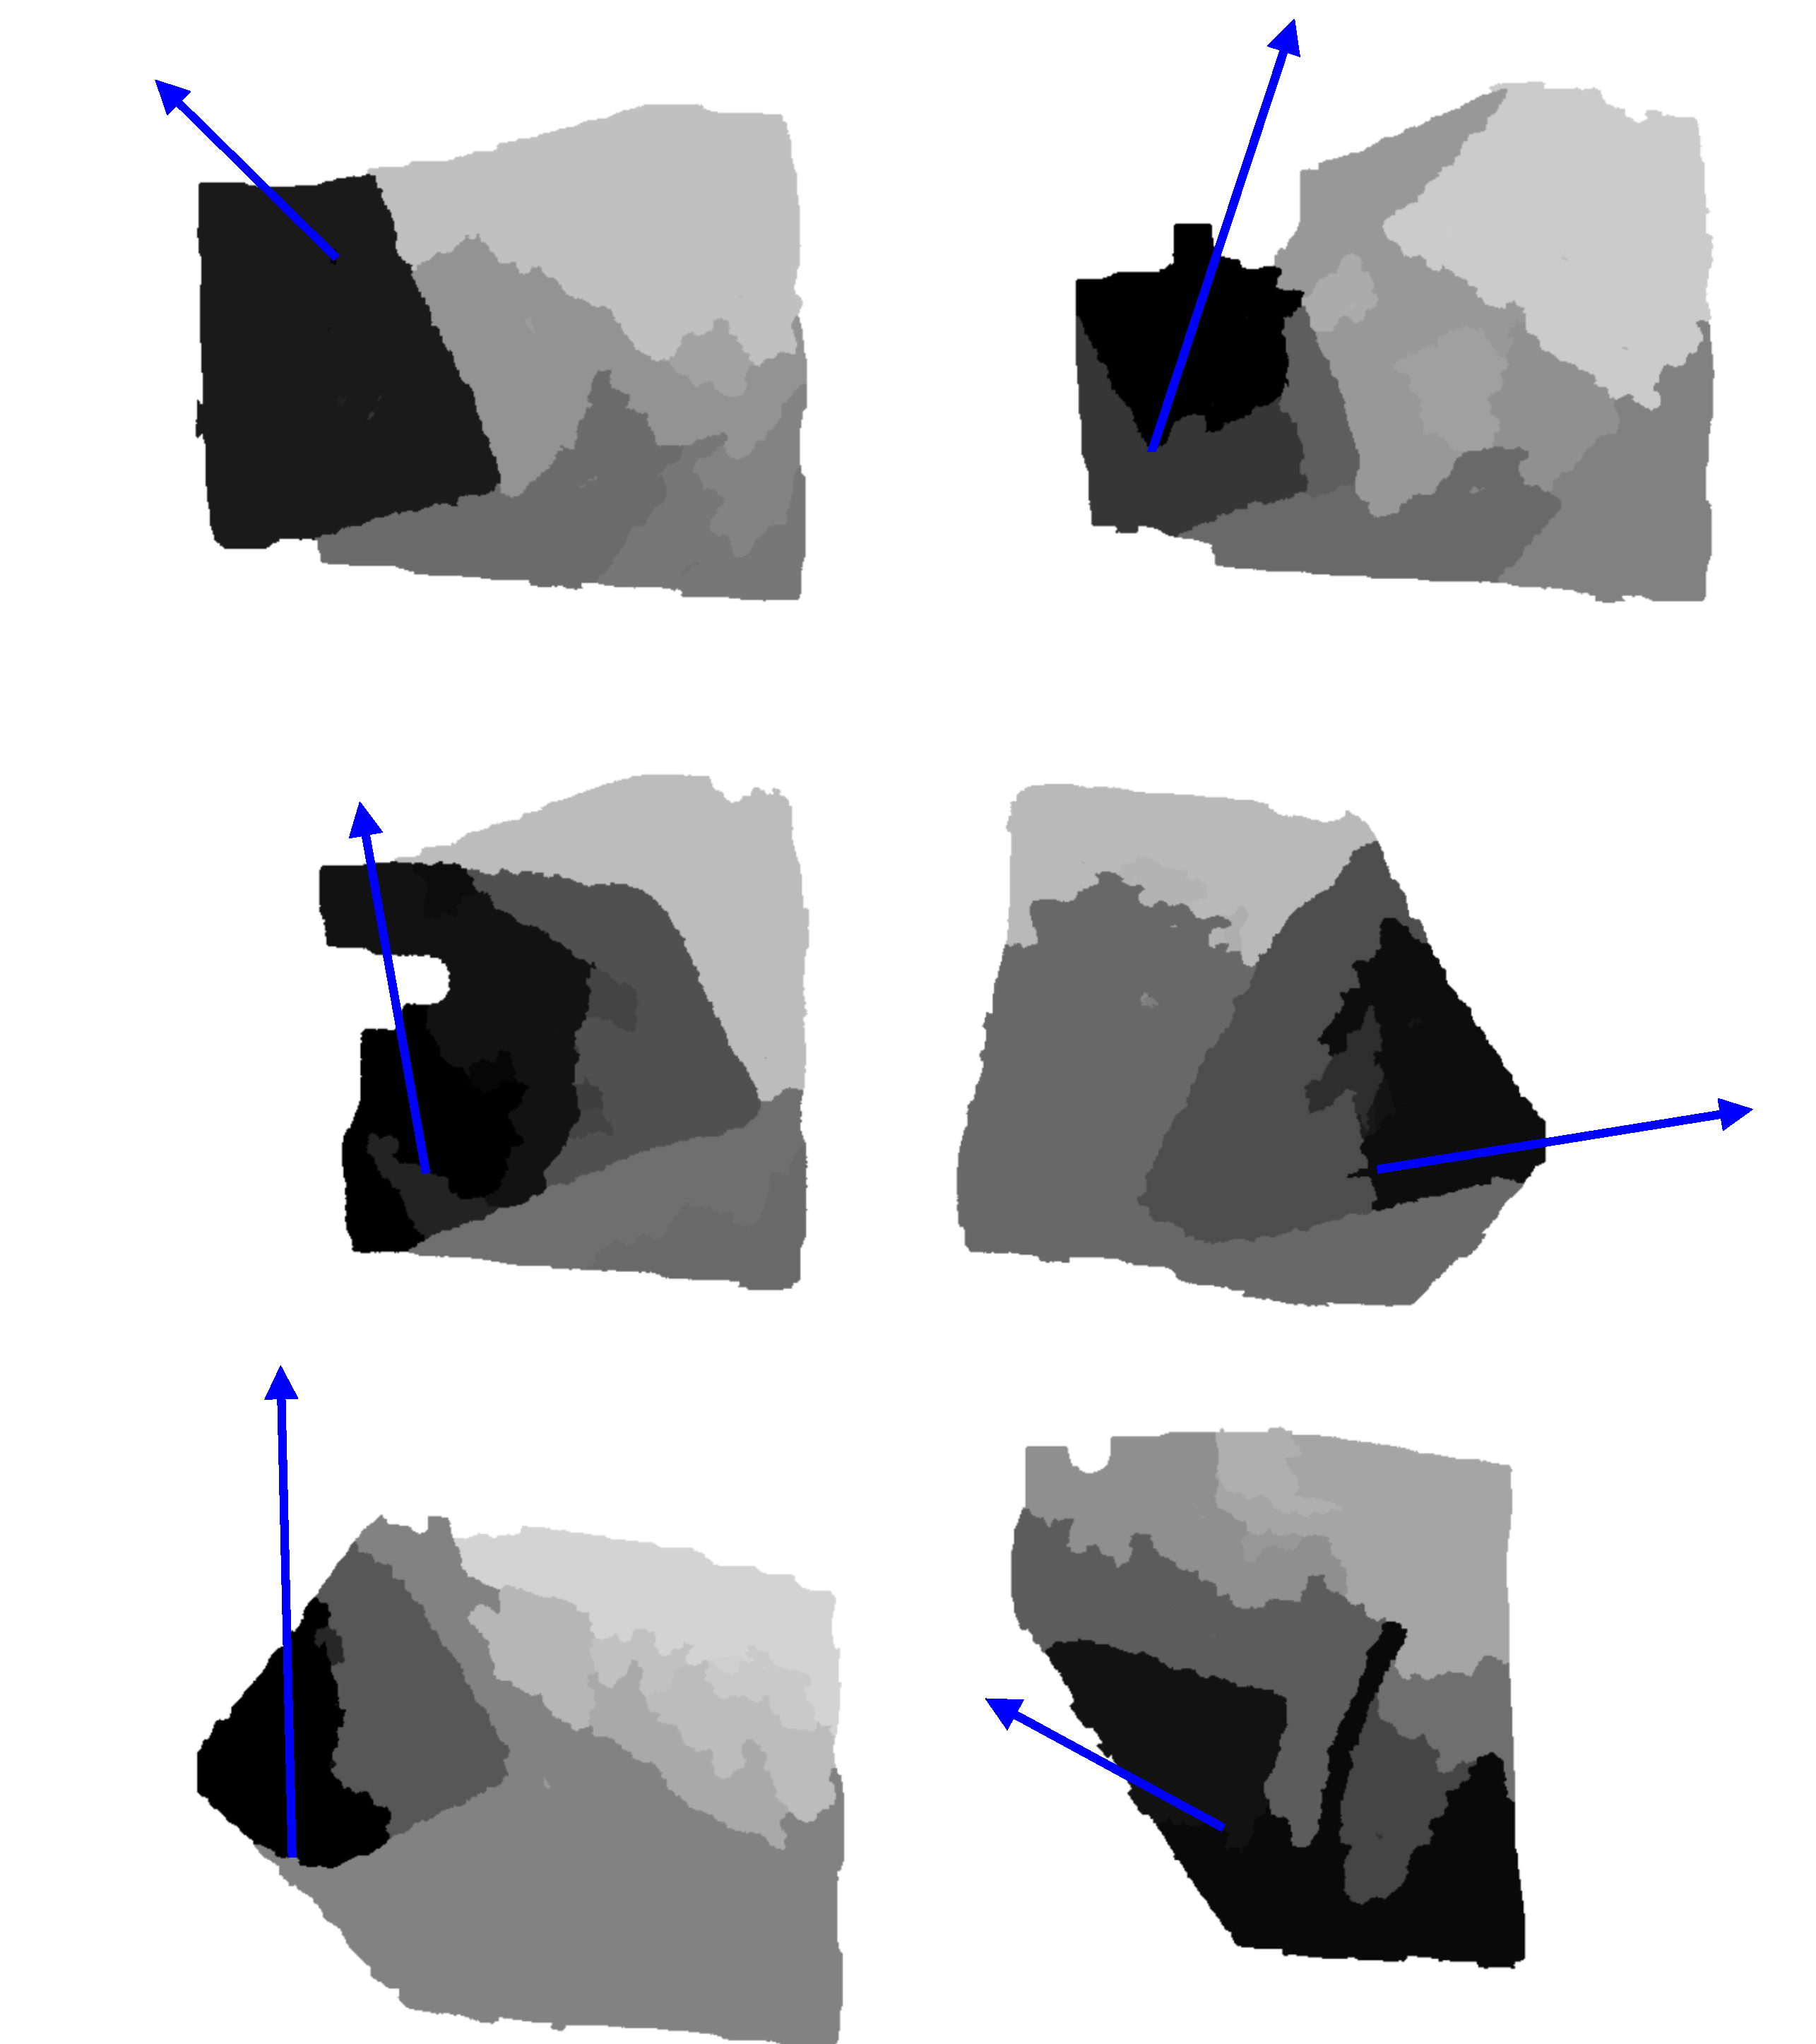
\includegraphics[width=\textwidth]
    {figures/directions.pdf}
    \caption[Final directions calculated for each garment provided to the system.]
    {Final directions calculated for each garment provided to the system. Each arrow departs where the robot should pick the fold and arrives where it should be placed. Darker regions represent regions that are closer to the camera, whereas lighter regions represent regions of the garment further from the camera.}
    \label{fig:directions}
\end{figure}

\comment{Lorem ipsum dolor sit amet, consectetur adipiscing elit. Donec a diam lectus. Sed sit amet ipsum mauris. Maecenas congue ligula ac quam viverra nec consectetur ante hendrerit. Donec et mollis dolor. Praesent et diam eget libero egestas mattis sit amet vitae augue. Nam tincidunt congue enim, ut porta lorem lacinia consectetur. Donec ut libero sed arcu vehicula ultricies a non tortor. Lorem ipsum dolor sit amet, consectetur adipiscing elit. Aenean ut gravida lorem. Ut turpis felis, pulvinar a semper sed, adipiscing id dolor. Pellentesque auctor nisi id magna consequat sagittis. Curabitur dapibus enim sit amet elit pharetra tincidunt feugiat nisl imperdiet. Ut convallis libero in urna ultrices accumsan. Donec sed odio eros. Donec viverra mi quis quam pulvinar at malesuada arcu rhoncus. Cum sociis natoque penatibus et magnis dis parturient montes, nascetur ridiculus mus. In rutrum accumsan ultricies. Mauris vitae nisi at sem facilisis semper ac in est.}

